% !TeX program = lualatex -synctex=1 -interaction=nonstopmode --shell-escape %.tex

\documentclass[_DKB_p1_Money.tex]{subfiles}
\begin{document}

\setbeamercovered{invisible}

\subsection{Ставка процента}
\begin{frame}[shrink=15]
\begin{figure}
\center
	\begin{overprint}
	\forloop{slideno}{1}{\value{slideno} < 2}{%
		\only<\value{slideno}>{
			\includegraphics[page=\value{slideno},
			scale=.7
			% trim={<left> <lower> <right> <upper>}				
			,trim={1cm 4cm 4cm 0cm},clip]
			{tikz/interest_rate_determination}}}
\end{overprint}
\vspace*{-1.5em}
\caption{Определение рыночной ставки процента}
\end{figure}
$r$ - реальная процентная ставка, (\%); 

$Q$ - предложение кредита и спрос на кредит в единицу времени;

$S$ - предложение кредита;

$D$ - спрос на кредит.
\end{frame}

\begin{frame}[allowframebreaks]{Номинальная и реальная процентные ставки}
\begin{block}{Процентная ставка }
\quad
— это цена кредита, которая распределяет кредит между домашними хозяйствами и фирмами.
\end{block}

\pagebreak
\begin{block}{Номинальная процентная ставка }
\quad
определяется как обменный курс, по которому текущие рублевые стоимости обмениваются на рублевые стоимости в будущем. 
\end{block}

\pagebreak
\begin{block}{Реальная процентная ставка }
\quad
— это обменный курс, по которому сегодняшние товары и услуги  обмениваются на товары и услуги в будущем. 
\end{block}

В мире без инфляции или дефляции номинальная процентная ставка равна реальной. 

\end{frame}

\begin{frame}[allowframebreaks]{\setfontsize{12pt}Зависимость между номинальной и реальной процентными ставками }
\begin{align}
r_n=r_r+\tau+(r_r \cdot \tau)
\end{align}
где

$r_n$ - номинальная процентная ставка;

$r_r$ - реальная процентная ставка;

$\tau$ - ожидаемые темпы инфляции.

\pagebreak
Предполагая, что процентные ставки и темпы инфляции относительно малы, можно записать уравнение в упрощенном виде
\begin{align}
r_n&=r_r+\tau\\
&\text{отсюда} \nonumber\\
r_r&=r_n-\tau
\end{align}

\end{frame}

\begin{frame}
\begin{figure}
\center
	\begin{overprint}
	\forloop{slideno}{1}{\value{slideno} < 3}{%
		\only<\value{slideno}>{
			\includegraphics[page=\value{slideno},
			scale=.6
			% trim={<left> <lower> <right> <upper>}				
			,trim={1cm 3cm 4cm 0cm},clip]
			{tikz/inflation_expectations}}}
\end{overprint}
\vspace*{-2em}
\caption{Инфляционные ожидания 4\%}
\end{figure}

Номинальная процентная ставка, $r_n$, увеличится из-за инфляционных ожиданий до $r_n + 4\%$.


\end{frame}

\begin{frame}{Виды процентных ставок}
\begin{itemize}
\item
Процентная ставка по корпоративным облигациям.
\item
Процентные ставки на межбанковском кредитном рынке.
\end{itemize}
\end{frame}

\subsection{Процентный доход}
\begin{frame}[allowframebreaks]{Расчет процентного дохода}
Номинальная доходность облигаций:
\begin{align}
r_n=\frac{C}{F}, 
\end{align}

где

\textit{C} - ежегодный купонный доход;

\textit{F} - номинал облигации.

\pagebreak
Текущая доходность облигаций:
\begin{align}
r_c=\frac{C}{P},
\end{align}

где

\textit{P} - рыночная цена облигации.

\end{frame}

\begin{frame}{Доходность при погашении долгосрочных облигаций}
Текущая стоимость любого актива в   будущем может быть задана уравнением:
\begin{align}
P=\frac{R_1}{1+r}+\frac{R_2}{(1+r)^2}+\frac{R_3}{(1+r)^3}+...+\frac{R_n}{(1+r)^n}
\end{align}
где

\textit{Р} — дисконтированная стоимость, т. е. текущая стоимость или рыночная цена актива.

$R_n$ - доход, который должен быть получен через \textit{n} лет от настоящего момента.

\textit{r}  — рыночная доходность.
\end{frame}

\begin{frame}
Расчет рыночной цены облигации

Облигация номиналом 1000₽ дает доход 50₽ в год и имеет срок погашения 3 года. 

Если рыночная процентная ставка равна 10\%, какова текущая продажная цена облигации?
\end{frame}

\begin{frame}[shrink=15]
% Table generated by Excel2LaTeX from sheet 'Лист1'
\begin{table}[htbp]
	\caption{Доходность при погашении облигаций с годовой купонной доходностью 6\%}
  \centering
    \begin{tabular}{cccccc}
    	\toprule
    	       r,\%        &         \multicolumn{5}{c}{n}         \\
    	\cmidrule(lr){2-6} &   6   &  6.5  &   7   &  7.5  &   8   \\ \midrule
    	        7          & 95,17 & 94,85 & 94,54 & 94,24 & 93,95 \\
    	       7,2         & 94,24 & 93,86 & 93,49 & 93,14 & 92,8  \\
    	       7,4         & 93,31 & 92,88 & 92,46 & 92,05 & 91,66 \\
    	       7,6         & 92,4  & 91,91 & 91,44 & 90,98 & 90,54 \\
    	       7,8         & 91,5  & 90,96 & 90,43 & 89,92 & 89,44 \\
    	        8          & 90,61 & 90,01 & 89,44 & 88,88 & 88,35 \\ \bottomrule
    \end{tabular}%
  \label{tab:addlabel}%
\end{table}%

\end{frame}

\begin{frame}[shrink=20]{Приблизительная оценка доходности облигаций}{Вариант 1.}
Доходность к погашению (Yield to Maturity (YTM), анг.) многолетней облигации:
\begin{align}
r_{YTM;m}&=\frac{C+\frac{N-P}{n\cdot m}}{(N+P)/2}\\
r_{YTM}&=(1+r_{YTM;m})^m-1.
\end{align}
где

$r_{YTM;m}$ - доходность к погашению облигации за период выплаты купона (меньше года);

$r_{YTM}$ - доходность к погашению облигации, годовых;

$C$ - купонная выплата по облигации за один период (как правило, меньше года);

$N$ - номинал облигации;

$P$ - рыночная цена облигации;

$n$ - число лет до погашения облигации;

$m$ - количество выплат купонов по облигации в одном году.

\end{frame}

\begin{frame}[shrink=20]{Приблизительная оценка доходности облигаций}{Вариант 2.}
Доходность к погашению (Yield to Maturity (YTM), анг.) многолетней облигации:
\begin{align}
r_{YTM;m}&=\frac{C+\frac{N-P}{n\cdot m}}{(N + 2 \cdot P)/3}\\
r_{YTM}&=(1+r_{YTM;m})^m-1.
\end{align}
где

$r_{YTM;m}$ - доходность к погашению облигации за период выплаты купона (меньше года);

$r_{YTM}$ - доходность к погашению облигации, годовых;

$C$ - купонная выплата по облигации за один период (как правило, меньше года);

$N$ - номинал облигации;

$P$ - рыночная цена облигации;

$n$ - число лет до погашения облигации;

$m$ - количество выплат купонов по облигации в одном году.

\end{frame}

\subsection{Рынок облигаций}
\begin{frame}
\begin{figure}
\center
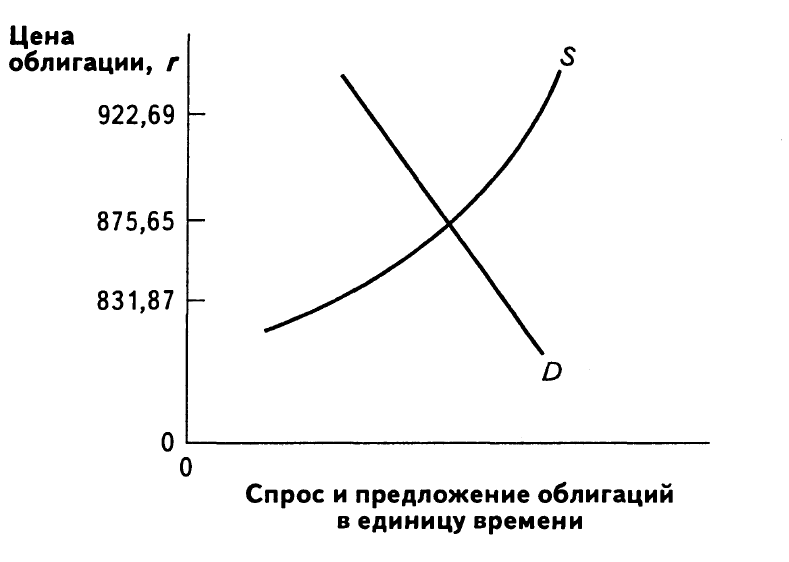
\includegraphics[scale=0.3]{img/ir_obligations_3y5per}
\caption{Рынок долгосрочных облигаций}
\end{figure}

Спрос и предложение 3-летних облигаций с номинальной доходностью 5\%. 

Равновесная цена установится на уровне 875,65₽, если рыночная процентная ставка равна 10\%.

\end{frame}

\begin{frame}{Доход по бессрочным облигациям (консолям)}
\begin{block}{Консоль }
\quad
– это облигация, которая имеет бесконечную продолжительность, т.е. никогда не будет погашена. Купонная доходность очередного выпуска устанавливается равной рыночной процентной ставке в день выпуска. Такие облигации выпускаются британским правительством 1 января каждого года.
\end{block}
\end{frame}
\begin{frame}
Рыночная цена консолей при известном купонном доходе и рыночной процентной ставке определяется по формуле:
\begin{align}
P=\frac{C}{r}
\end{align}

Где 

$r$ - рыночная процентная ставка;

$C$ - единовременная купонная выплата по облигации.
\end{frame}

\begin{frame}{}
\begin{figure}
\center
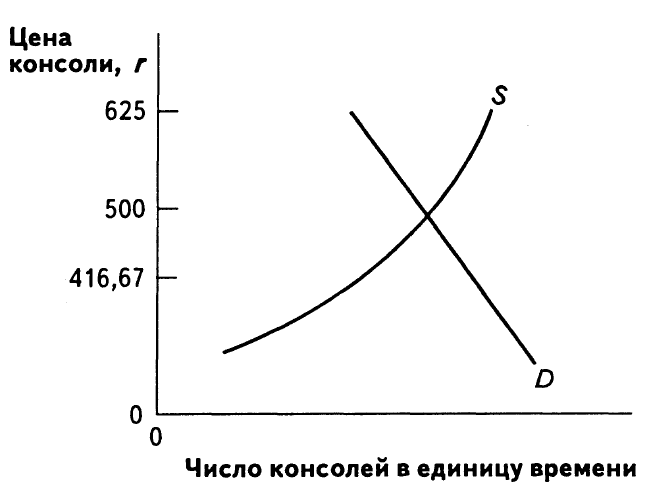
\includegraphics[scale=0.3]{img/ir_console}
\caption{Спрос и предложение консолей}
\end{figure}

Кривые спроса и предложения консолей с доходом 50₽ в год. 

Равновесие существует при цене 500₽, что эквивалентно рыночной процентной ставке 10\%.
\end{frame}

\setbeamercovered{invisible}
\begin{frame}[shrink=10]
Цены на облигации с различными сроками погашения
Номинал трехлетней облигации 1000₽. Ежегодный купонный доход как по трехлетней облигации, так и по консоли составляет 50₽.
% Table generated by Excel2LaTeX from sheet 'Лист3'
\begin{table}[htbp]
\caption{Изменение процентной ставки и цены на облигации}
  \centering
    \begin{tabular}{ccc}
    \toprule
    r, \% & \multicolumn{2}{c}{n} \\\cmidrule{2-3}
          & 3 & $\infty$ \\
    \midrule
    12    & \onslide<2->{831,87₽} & \onslide<5->{416,67₽} \\
    10    & \onslide<3->{875,65₽} & \onslide<6->{500,00₽} \\
    8     & \onslide<4->{922,69₽} & \onslide<7->{625,00₽} \\
    \bottomrule
    \end{tabular}%
  \label{tab:addlabel}%
\end{table}%
\end{frame}

\begin{frame}{Кривая доходности}
\begin{figure}
\center
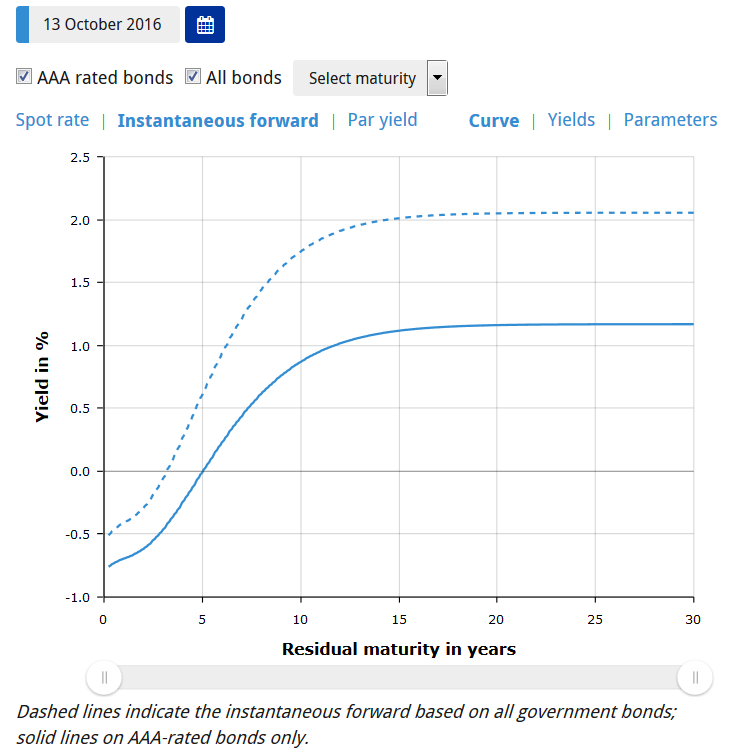
\includegraphics[scale=0.25]{img/yield_curve.png}
\caption{Доходность по облигациям правительств европейских стран}
\end{figure}
Источник: \href{http://www.ecb.europa.eu/stats/money/yc/html/index.en.html}{Европейский центральный банк. 2016.}
\end{frame}

\setbeamercovered{transparent}
\begin{frame}[allowframebreaks]{Государственные краткосрочные облигации}
Номинальная процентная ставка (ставка дисконта, вычисленная на основании 360-дневного года (такая длительность года принята для упрощения расчетов)):
\begin{align}
r_b=[(N-P)/N]\times (360/n)
\end{align}

где

N - номинал облигации;

P - рыночная цена облигации;

n - срок до погашения облигации в днях.

\pagebreak
Эквивалентный купонный доход:
\begin{align}
r_y=[(N-P)/P]\times (365/n)
\end{align}
\end{frame}

\setbeamercovered{invisible}
\begin{frame}
Облигация номиналом 10000~₽ со сроком погашения через 91 день продается на аукционе за 9685~₽. 

За 73 дня до погашения эта облигация продавалась на вторичном рынке по цене 9678,50~₽.

\onslide<2->{$r_b=12,462\%.$}

\onslide<3->{$r_y=13,046\%.$}

\onslide<4->{$r_y=16,608\%.$}
\end{frame}

\setbeamercovered{transparent}

\begin{frame}[ allowframebreaks]{Ликвидность и государственные облигации}
Удвоение процентных ставок в экономике.

Имеются две облигации номиналом 1000~₽ каждая и сроками 91 день и 5 лет соответственно. По пятилетней облигации выплачивается ежегодный купон 50~₽. В момент выпуска доходность по обеим бумагам была равна 10\%. Определите рыночные цены этих облигаций.

\pagebreak
На следующий день процентные ставки на рынке уменьшились в два раза. Определите как изменились цены на эти облигации на вторичном рынке.

Рассчитайте изменение цен на эти облигации в случае удвоения процентных ставок.
\end{frame}







\setbeamercovered{transparent}
\end{document}